%%This is a very basic article template.
%%There is just one section and two subsections.
\documentclass[12pt]{article}
\usepackage[paper=a4paper,left=20mm,right=20mm,top=30mm,bottom =30mm]{geometry}
\usepackage[utf8]{inputenc}
\usepackage[T1]{fontenc}
\usepackage{stmaryrd}
\usepackage{setspace}
\usepackage{mathrsfs}
\usepackage[ngerman]{babel}
\usepackage{amssymb}
\usepackage{amsmath}
\usepackage{fancyhdr}
\usepackage[dvips,unicode,colorlinks,linkcolor=black]{hyperref} 
\usepackage{graphicx}
\usepackage{float}

\pagestyle{fancy}
\lfoot{}
\rfoot{Paul Kremser, Tobias Grussenmeyer}
\cfoot{\thepage}
\fancyhead[L]{FPI Versuch: Ringlaser}
\renewcommand{\headrulewidth}{0.6pt}
\renewcommand{\footrulewidth}{0.6pt}
\setlength{\headheight}{16pt}
\setlength{\parindent}{0pt}
% Für die Wahl der Schriftart
\newcommand{\changefont}[3]{
\fontfamily{#1} \fontseries{#2} \fontshape{#3} \selectfont}

\begin{document}
% keine Hurenkinder und Schusterjungen
\clubpenalty = 10000
\widowpenalty = 10000 
\displaywidowpenalty = 10000

\onehalfspacing
% Schriftart
\changefont{ptm}{m}{n} 

\begin{titlepage}
\author{Paul Kremser, Tobias Grussenmeyer}
\title{Versuch: Ringlaser}
\date{Versuchsdurchführung: 1. und 2. Oktober 2009} 
\maketitle
\thispagestyle{empty}
\end{titlepage}


\tableofcontents
\thispagestyle{empty}
\newpage
\pagenumbering{arabic}
\section{Überblick}
Mit Hilfe eines Ringlasers soll der Mitführungskoeffizient bestimmt werden.
Hierzu wird der Laserstrahl durch eine schräg stehende rotierende Quarzscheibe geführt. Dies hat zur Folge,
dass rechts- und linksumlaufende Welle veränderte optische Weglängen vorfinden. Durch Messung der daraus resultierenden
Frequenzdifferenz lässt sich der Mitführungskoeffizient bestimmen.

\section{Aufgabestellung}
\begin{itemize}
 \item Bestimmung des Mitführungskoeffizienten $\alpha$ durch Messung der Schwebungsfrequenz bei
\begin{enumerate}
 \item Variation des Durchtrittspunktes $x_0$ für 3 bis 4 feste Drehzahlen und
 \item Variation der Drehzahl für 3 bis 4 eingestellte Werte von $x_0$
\end{enumerate}
 \item Vergleich des experimentell gefundenen Werts fuer $\alpha$ mit dem aus dem Brechungsindex berechneten Wert.
\end{itemize}

\section{Theoretische Grundlagen}
Im Vakuum breitet sich Licht mit der konstanten Lichtgeschwindigkeit $c$ aus. Bei Ausbreitung von Licht in einem Medium hingegen
hängt die Geschwindigkeit vom Brechungsindex $n(\lambda)$ und der Relativgeschwindigkeit des Mediums ab.
\subsection{Mitführungskoeffizient}
Der Mitführungskoeffizient $\alpha$ lässt sich aus der Relatitätstheorie ableiten. Hierzu betrachte man zwei Systeme $K$ und $K'$ welche sich in $x$-Richtung
mit der Geschindigkeit $w$ voneinander entfernen. Für die Geschwindigkeit $v$ in $K$, eines Teilchens welches sich in $K'$ mit der Geschwindigkeit $v'$ 
in $x'$-Richtung bewegt, gilt nach der Lorenztransformation:
\begin{align}
 v = \frac{v' + w}{1 + v'\times\frac{w}{c^2}}
\end{align}

\begin{figure}[H]  
\centering
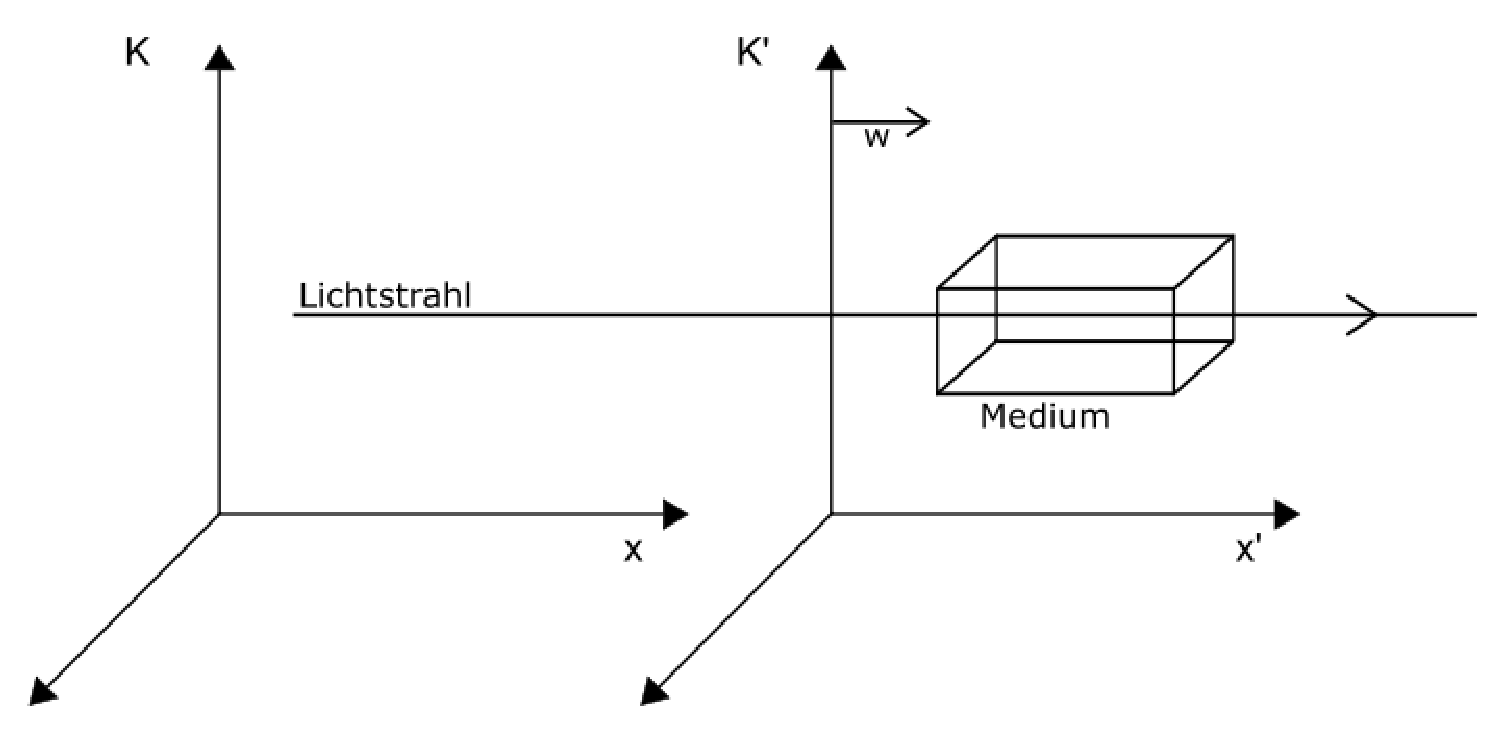
\includegraphics[width=0.9\linewidth]{pictures/abb1.eps}
\caption{Lichtstrahl in einem bewegten Medium}
\label{abb1}
\end{figure}

Betrachtet man nun ein Medium welches sich mit der Geschwindigkeit $\pm w$ relativ zu $K$ bewegt (siehe Abb.1), so ist die Geschindigkeit $v'$ 
eines Lichtstrahls welcher sich in $x$-Richtung ausbreitet gegeben durch $v' = \frac{c}{n}$ ($n$ Brechungsindex). Was sich in $K$ zu 
\begin{align}
 v = \frac{\frac{c}{n} \pm w}{1 \pm \frac{w}{c \ n}}
\end{align}
transformiert. Da $w \ll c$ kann man die Abschätzung $\frac{1}{1 \pm x} \approx (1 \mp x)$ für $x \ll 1$ machen und erhält:
\begin{align}
 v &\approx \left( \frac{c}{n} \pm w\right) \left( 1 \mp \frac{w}{c \ n}\right) = \frac{c}{n} \pm \left( 1 - \frac{1}{n^2} \mp \frac{w}{c \ n}\right) w \\
 \label{fresneldreck}  &\approx \frac{c}{n} \pm \left( 1 - \frac{1}{n^2}\right) w = \frac{c}{n} \pm \alpha \ w
\end{align}

Erstaunlicherweise wurde selbige Formel bereits Anfang des 19ten Jahrhunderts von Frensel gefunden. Dieser ging allerdings von der Existenz eines 
Äthers aus und hatte die Vorstellung das der Äther von der Bewegung des Mediums mitgeführt würde.
Daher nennt man diese Formel auch Mitführungsformel und $\alpha$ dem Mitführungskoeffizient.


%Fresnel
\subsection{Der Dispersionsterm}
In der Fresnelschen Mitführungsformel wurde die Frequenzabhängigkeit des Brechungsindex noch nicht berücksichtigt.
Da das Meium mit der Geschwindigkeit $w_i$ gegenüber dem einfallenden Lichtstrahl bewegt wird, ist hier der Dopplereffekt zu berücksichtigen. Die relativistische Dopplerformel liefert für $w_i \ll c$:
\begin{align}
 \label{doppler}\nu' = \nu \left(1 \mp \frac{w_i}{c}\right)
\end{align}

Nähert man $n(\nu')$ bis zum linearen Glied und setzt Gleichung \ref{doppler} ein, so erhält man:
\begin{align}
 n(\nu')=n(\nu)+(\nu'-\nu)\frac{dn(\nu)}{d\nu}=n(\nu)\ \left(1\mp\frac{w_i}{c}\frac{\nu}{n(\nu)}\frac{dn(\nu)}{d\nu}\right)
\end{align}

Setzt man dies in Gleichung \ref{fresneldreck} ein so erhält man:
\begin{align}
 v &\approx \frac{c}{n(\nu')} \pm \left( 1-\frac{1}{(n(\nu'))^2}\right) w \\
 &\approx \frac{c}{n(\nu} \left( 1 \mp \frac{w_i \nu}{cn(\nu)} \frac{dn(\nu}{d\nu} \right) ^{-1} \pm w \left( 1-\frac{1}{(n(\nu))^2} \left( 1 \mp \frac{w_i \nu}{cn(\nu)}\frac{dn(\nu)}{d\nu} \right) ^{-2} \right)
\end{align}

Nähert man $(1\mp x)^{-1} \approx (1\pm x)$ und $(1\mp x)^{-2} \approx (1\pm 2x)$ für $x \ll 1$ folgt wegen $w\ll c$:
\begin{align}
 \nu \approx \frac{c}{n} \left( 1 \pm \frac{w_i\nu}{cn} \frac{dn}{d\nu} \right) \pm w \left( 1- \frac{1}{n^2} \left( 1 \pm 2 \frac{w_i \nu}{cn} \frac{dn}{d\nu} \right) \right) \textnormal{  mit } n \equiv n(\nu)
\end{align}

und weiter:
\begin{align}
 \nu \approx \frac{c}{n} \pm w \left( 1- \frac{1}{n^2} \right) \pm \frac{w_i \nu}{n^2} \frac{dn}{d\nu} = \frac{c}{n} \pm \left( 1- \frac{1}{n^2} + \frac{w_i}{w} \frac{\nu}{n^2} \frac{dn}{d\nu} \right)
\end{align}

Berücksichtigt man $\lambda = c/\nu$ folgt hieraus:
\begin{align}
 \label{dragcomplete} v \approx \frac{c}{n} \pm w \left( 1- \frac{1}{n^2} - \frac{w_i}{w} \frac{\lambda}{n^2} \frac{dn}{d\lambda} \right)
\end{align}

\begin{figure}[H]  
\centering
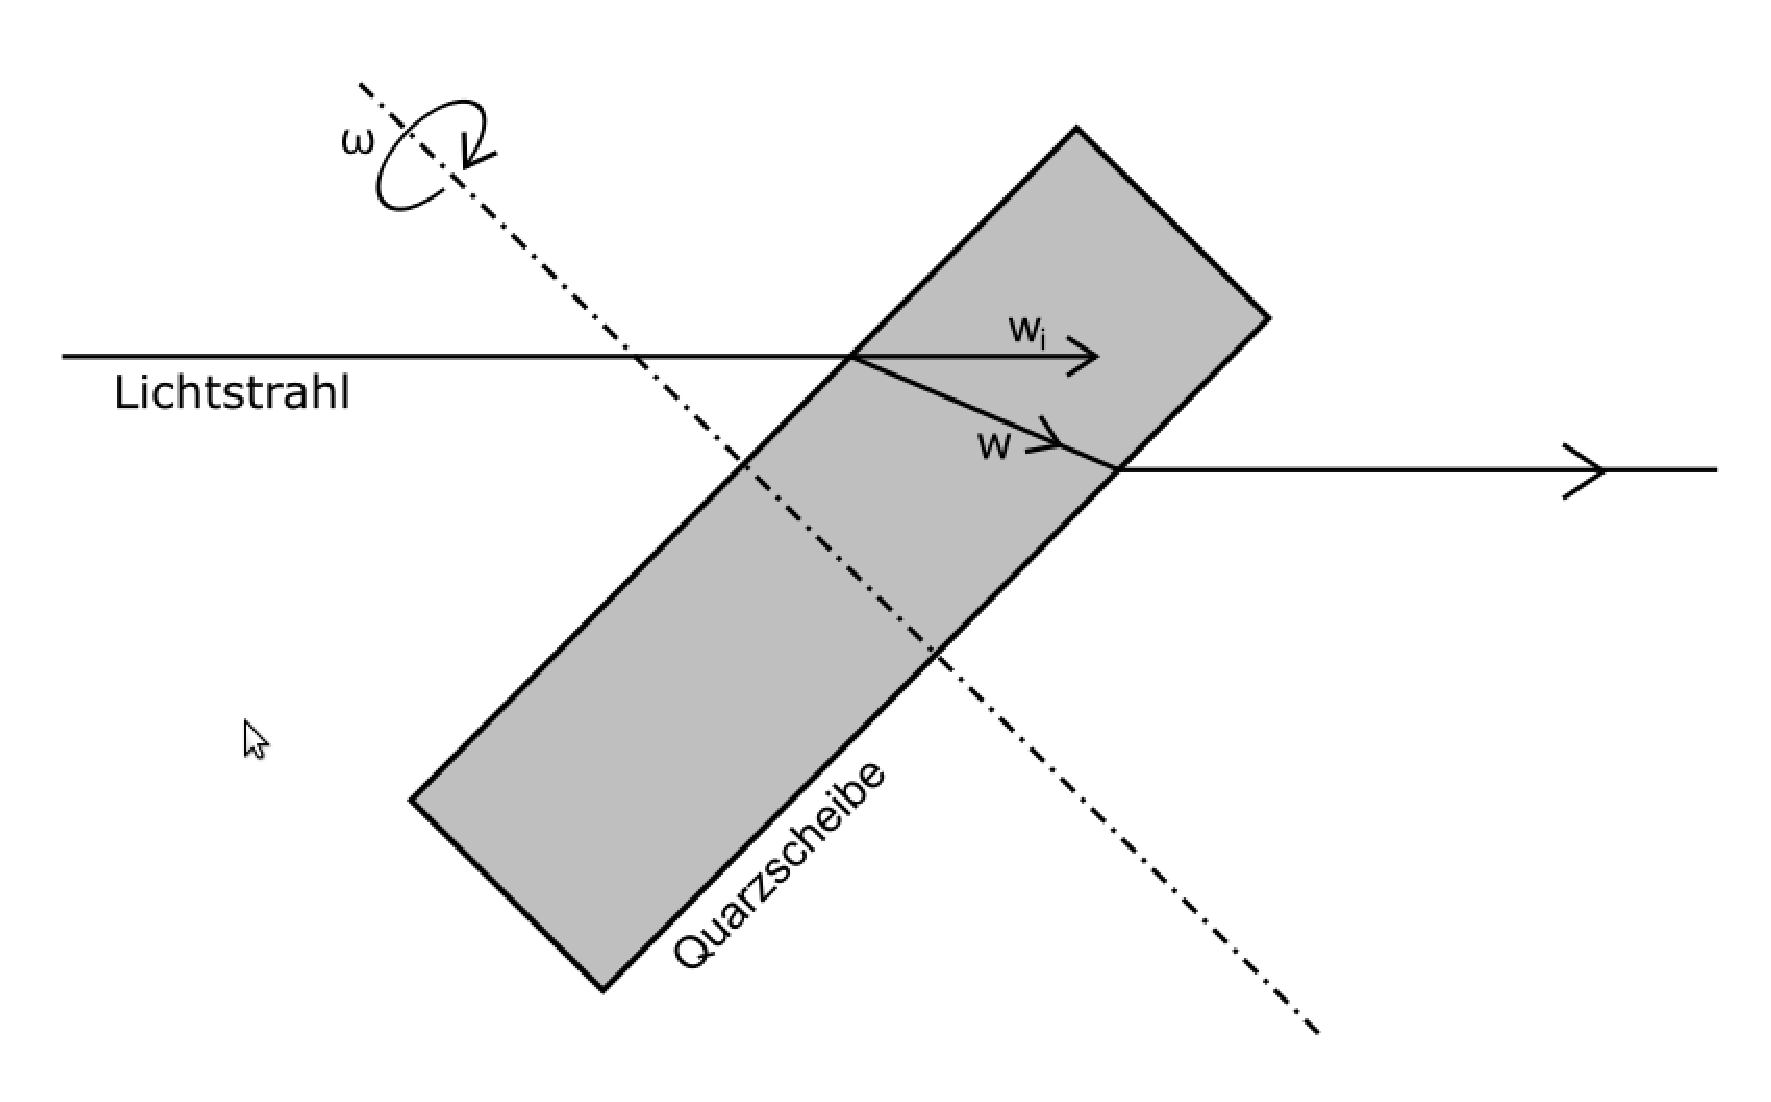
\includegraphics[width=0.9\linewidth]{pictures/abb3.eps}
\caption{Lichtstrahl fällt durch eine rotienende Quarzscheibe}
\label{abb3}
\end{figure}

In unserer Anordnung (siehe Abb. \ref{abb3}) unterscheidet sich die Geschwindigkeitskomponente $w$ der Quartzscheibe in Richtung des gebrochenen Strahls von der Komponente $w_i$ in Richtung des einfallenden Strahls. Dabei sind diese Komponenten über den Brechungsindex verknüpft, es gilt:
\begin{align}
 \frac{w_i}{w}=n
\end{align}

eingesetzt in Gleichung \ref{dragcomplete} folgt daraus:
\begin{align}
 v=\frac{c}{n} \pm w \left(1-\frac{1}{n^2} - \frac{\lambda}{n} \frac{dn}{d\lambda} \right)
\end{align}

Vergleicht man dies mit Gleichung \ref{fresneldreck} sieht man das zu dem Mitführungskoeffizienten noch ein zusätzlicher Term 
\begin{align}
 -\frac{\lambda}{n} \frac{dn}{d\lambda}
\end{align}

hinzugekommen ist. Dieser wird auch \textit{Dipersionsterm} genannt. Also erhalten wir für unsere Anordnung den Mitführungskoeffizienten 
\begin{align}
\label{mitfuehrung} \alpha = 1 - \frac{1}{n^2} - \frac{\lambda}{n} \frac{dn}{d\lambda}
\end{align}


\subsection{Frequenzunterschied zwischen links- und rechtsumlaufender Welle}
Durch die Geschwindigkeitskomponente der Bewegung der Quarzscheibe entlang des Lichtstrahls erscheint das Medium für den links- bzw. rechtsumlaufenden
Strahl dichter bzw. weniger dicht. Dies bedeutet also einen Unterschied im Brechungsindex und somit einen Unterschied der optischen Wege. Durch Überlagerung
von links- und rechtsumlaufender Welle bildet sich im Ringlaser eine Stehende Welle für die folgendes gilt:
\begin{align}
 N \ \lambda = L \quad \textnormal{mit} \ N \in \mathbb N \quad \textnormal{und} \ L = \sum_{i}{n_i \ l_i} \ \textnormal{,}
\end{align}
wobei $L$ die optische Weglänge des Aufbaus ist und $l_i$ die längen der Wegstrecken mit Brechungsindex $n_i$ sind,
aus.

Für kleine Längenänderungen bleibt das System in der selben Schwingungsmode, d.h. $N = const$ und $dL = N \ d\lambda$. Für kleine $\Delta L$ gilt somit:
\begin{align}
 \frac{\Delta L}{L} = \frac{\Delta\lambda}{\lambda} = -\frac{\Delta \nu}{\nu}
\end{align}

Der Geschwindigkeitsunterschied der beiden Strahlen ist $2 \ \alpha \ w$. Wenn $n \ l$ der optische Weg im ruhenden Medium ist, folgt:
\begin{align}
 \frac{\Delta (l \ n)}{l \ n} = \frac{v(w \neq 0) - v(w = 0)}{v(w = 0)} = \frac{\frac{c}{n} \pm \alpha \ w - \frac{c}{n}}{\frac{c}{n}}
 = \pm \frac{n \ \alpha \ w}{c}
\end{align}

Da die Änderung $\Delta L$ des optischen Wegs des Systems durch die Änderung des optischen Wegs im Medium gegeben ist, also durch
$\Delta L = \Delta(l \ n)$, folgt:
\begin{align}
 \frac{\Delta L}{L} = \frac{l \ n}{L} \frac{\Delta(l \ n)}{l \ n} = \pm \frac{n^2 \ \alpha \ l \ w}{L \ c} = -\frac{\Delta \nu}{\nu}
\end{align}

und für den gemessenen Frequenzunterschied der beiden Strahlen bekommt man:
\begin{align}
\label{nuexp} \Delta\nu_{exp} = 2 \Delta\nu = \frac{2 \ n^2 \ \alpha \ l \ w \ \nu}{L \ c} = \frac{2 \ n^2 \ \alpha \ l \ w}{\lambda \ L}
\end{align}

Mittels etwas komplizierten Überlegungen (siehe Staatsex. ...) kann man $w$ und $l$ durch die Parameter der Rotierenden Quarzscheibe
(Winkelgeschwindigkeit $\omega$, Strahleintrittspunkt $x_0$, Dicke der Scheibe $d$ und Brechungsindex $n$) ausdrücken:
\begin{align}
 w \ l = \frac{d \ x_0 \ \omega}{n}
\end{align}

Durch Einsetzten in Gl. \ref{nuexp} bekommt man für den Mitführungskoeffizienten:
\begin{align}
\label{mitfuehrungskoeff} \alpha = \frac{\Delta\nu_{exp} \ \lambda \ L}{2 \ n \ d \ x_0 \ \omega}
\end{align}


\section{Versuchsaufbau}
Der Ringlaser besteht aus drei an den ecken eines gleichseitigen Dreiecks aufgestellten Spiegeln. Zwischen zwei dieser Spielgel befindet sich eine He-Ne-Entladungsrohr.
In einem weiteren Arm der Anordnung befindet sich die rotierbare Quarzscheibe, diese wird über einen Gummiriemen mittels eines Motors angetrieben.
Ebenso im Strahlengang befindet sich eine um 180 zur rotierenden Quarzscheibe gedrehte zweite Quarzscheibe der gleichen Dicke um die Verschiebung des Strahls
an der ersten Scheibe auszugleichen. Der Laserstrahl trifft unter dem Brewsterwinkel in den Quarz ein um Refelxtionen gering zu halten.
Die beiden Scheiben sind auf einem beweglichen Schlitten gelagert dessen Position mit einer Mikrometerschraube eingestellt
werden kann. 

Um die Rotationsgeschwindigkeit der Quarzscheibe festzustellen befindet sich eine Lichtschranke an der Scheibe die an einen Zähler angeschlossen ist.
Der Zähler zeigt die Umlaufdauer in $\mu$s an.

Im Resonator können sich rechts- und linksumlaufende Wellen ausbilden. Bei ruhender Quarzscheibe haben beide den selben optischen Weg, dreht sich jedoch 
die Scheibe so erhält man unterschiedliche Weglängen für die beiden Richtungen was sich in unterschiedlichen Frequenzen für die Umlaufsinne auswirkt.
Dieser Frequenzunterschied kann als Schwebung mit einer Photodiode gemessen werden. Hierzu wird bei Spiegel $S_3$ ein kleiner Teil des Signals ausgekoppelt
und mit hilfe von $S_4$ werden beide Strahlen auf der Photodiode überlagert.

Um möglichst wenige Moden auf dem Oszilloskop sichtbar zu machen ist im Strahlengang eine Blende montiert. Ohne diese wäre die Messung nicht möglich da
man sonst eine irreguläre Darstellung aus Anteilen vieler verschiedener Moden erhalten würde.

\begin{figure}[H]  
\centering
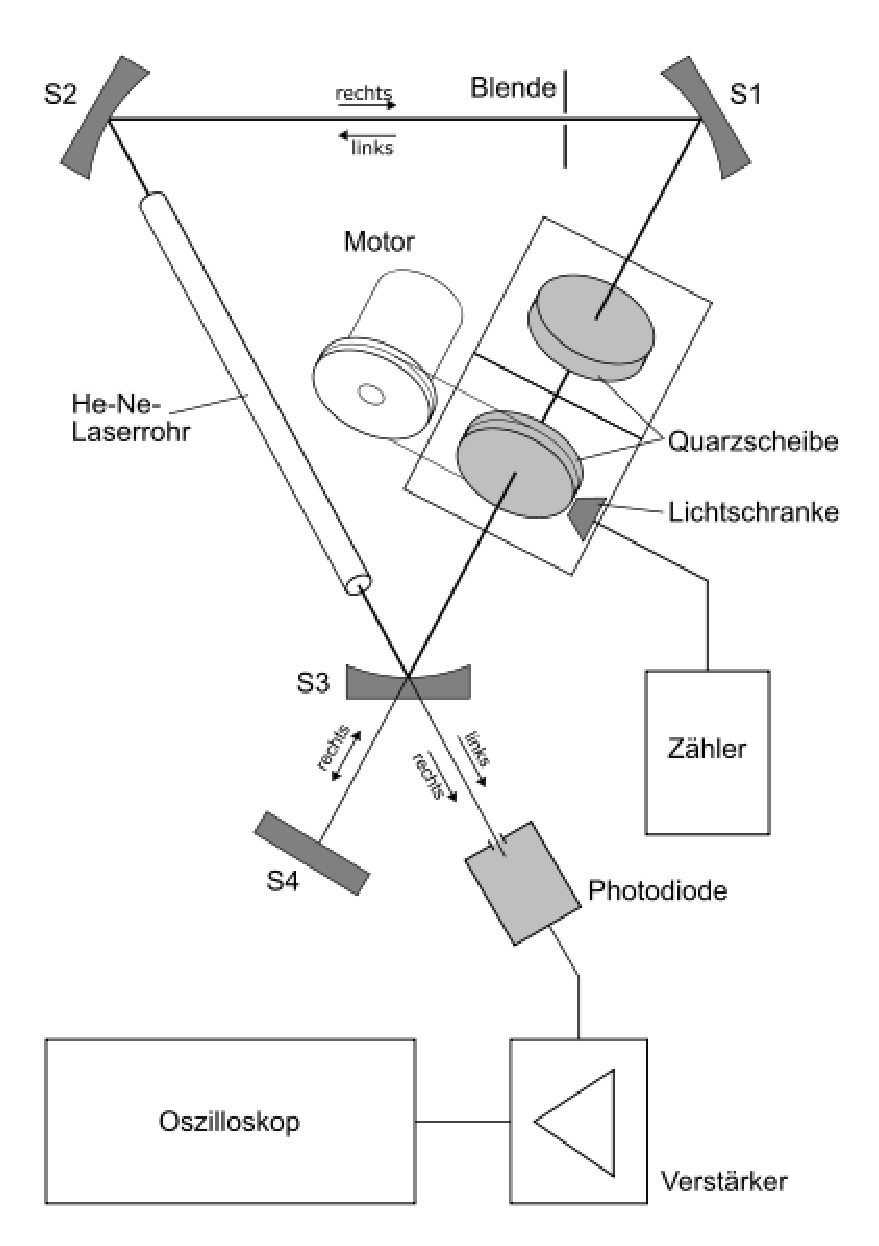
\includegraphics[width=0.7\linewidth]{pictures/abb4.eps}
\caption{Versuchsanordnung Ringlaser}
\label{versuchsaufbau}
\end{figure}

\section{Durchführung}
Nach der Justierung der Blende und des Auskopplungsspiegels konnte man auf dem Oszilloskop das Signal, welches sich leider nicht so triggern lässt das es 
still steht, sinusähnliche Formen annimmt. Mittels der Hold-Funktion des Oszilloskops konnte man ein Bild auswählen bei welchem die Wellenform eine
Bestimmung der Frequenz zulässt. 

Wir unternahmen 3 Messreihen mit konstanter Drehzahl der Quarzscheibe unter Variation des Eintrittspunktes des Strahls auf der Scheibe und 3 Messreihen
mit festem Eintrittspunkt bei Variation der Drehzahl.
\section{Auswertung}


\subsection{Variation der Drehzahl}
Bei den Messreihen mit Variation der Drehzahl haben wir jeweils die Schwebungsfrequenz $\Delta\nu_{exp}$ gegen die Winkelgeschwindigkeit $\omega$
aufgetragen. Wie sich $\omega$ und $\Delta\nu_{exp}$ und deren Fehler berechnen wurde bereits im Abschnitt Variation des Durschtrittspunktes behandelt.

Nach Gleichung \ref{mitfuehrungskoeff} gilt:
\begin{align}
 \Delta\nu_{exp} = \frac{2 \ n \ d \ x_0 \ \alpha}{L \ \lambda}
\end{align}

Mit hilfe einer linearen Regression $\Delta\nu_{exp} = p_0 + p_1 \ \omega$ lässt sich also $\alpha$ bestimmen:
\begin{align}
 \alpha = \frac{L \ \lambda \ p_1}{2 \ n \ d \ x_0}
\end{align}

wobei $x_0$ aus dem in der Messung, mit Variablem Durchtrittspunkt, bestimmten Mittelpunkt $x_m$ bestimmt haben.
Mit Gauß erhält man für den Fehler auf $\alpha$:
\begin{align}
 s_{\alpha} = \lvert \alpha \rvert \sqrt{\left(\frac{s_{p_1}}{p_1}\right)^2 + \left(\frac{s_{x_0}}{x_0}\right)^2}
\end{align}

Von den Werten für $\alpha$ aus den 3 Messreihen bildeten wir das gewichtete Mittel:
\begin{align}
 \alpha = x \ \pm \ x
\end{align}





\begin{figure}[H]  
\centering
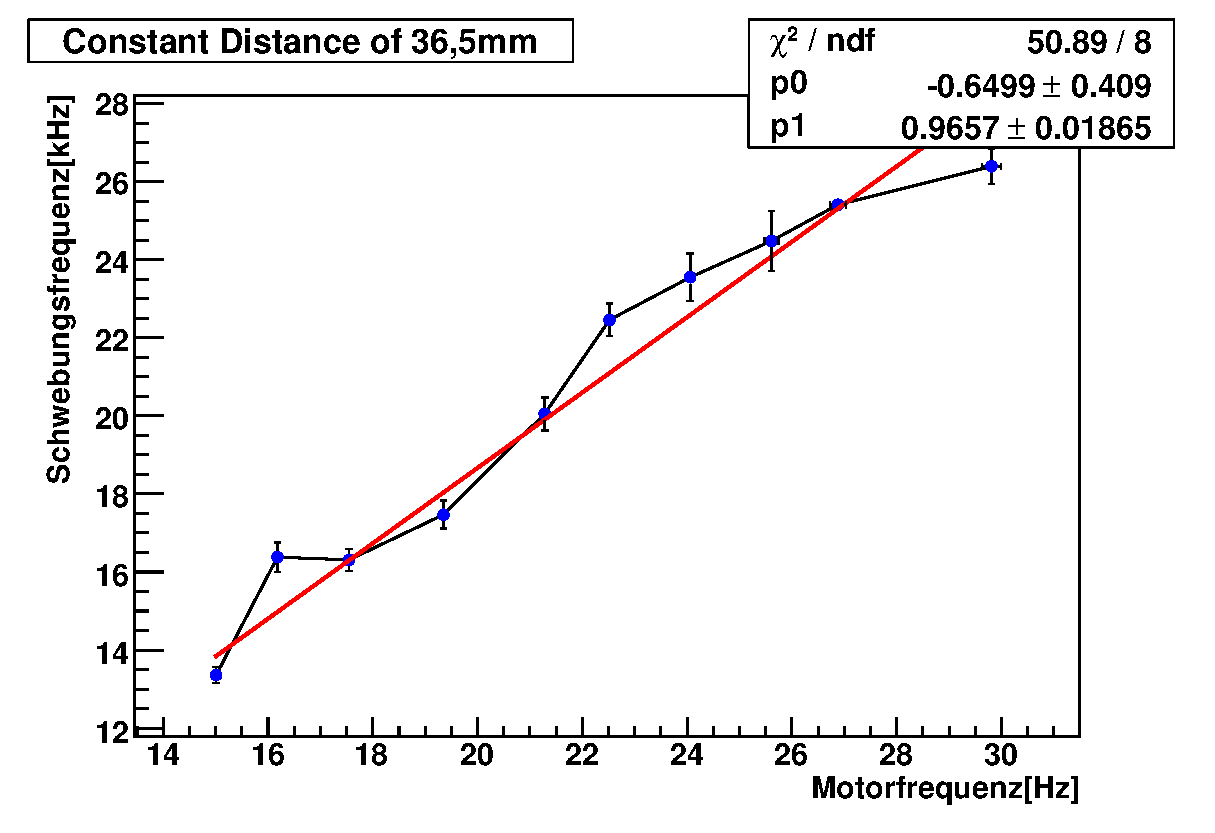
\includegraphics[width=0.7\linewidth]{pictures/36,5mm1.eps}
\caption{Messreihe bei $x_0 = 36,5mm$ mit variabler Drehzahl}
\label{36mm}
\end{figure}

\begin{figure}[H]  
\centering
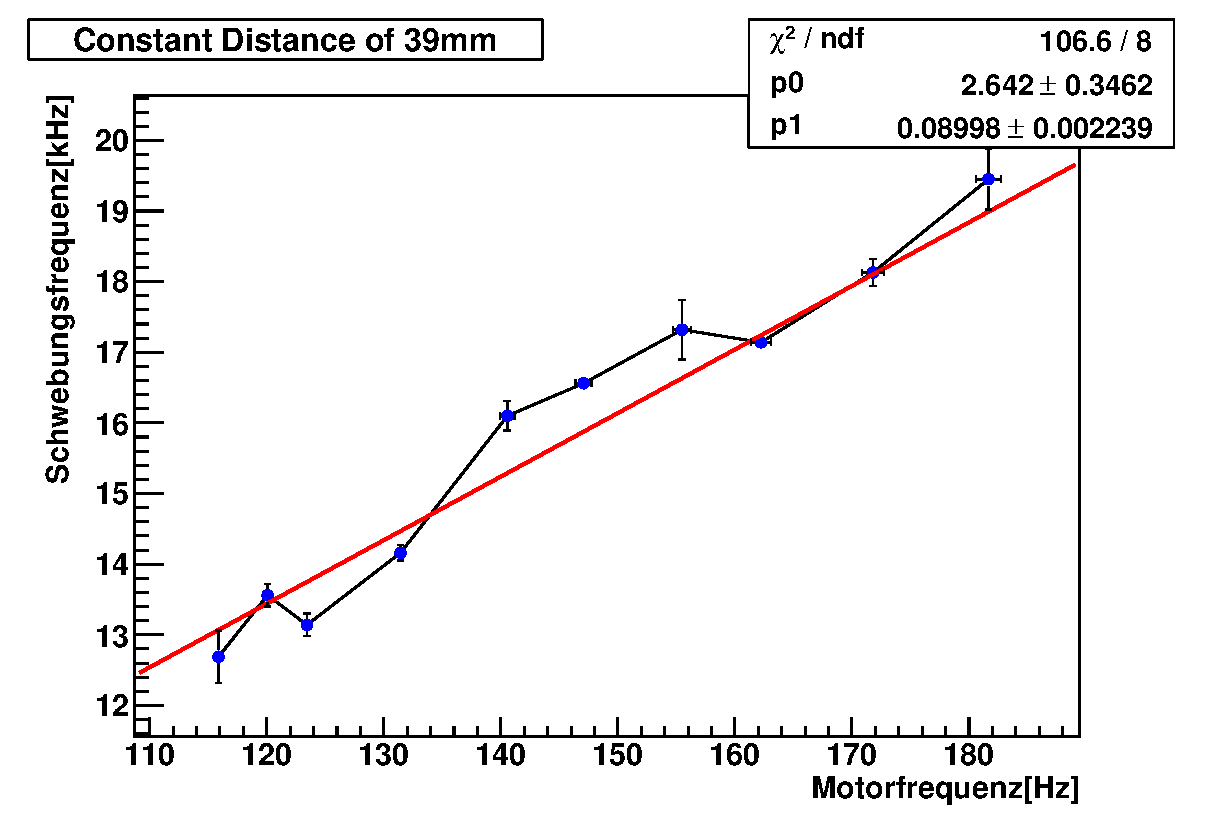
\includegraphics[width=0.7\linewidth]{pictures/39mm1.eps}
\caption{Messreihe bei $x_0 = 39mm$ mit variabler Drehzahl}
\label{39mmm}
\end{figure}

\begin{figure}[H]  
\centering
\includegraphics[width=0.7\linewidth]{pictures/55mm1.eps}
\caption{Messreihe bei $x_0 = 55mm$ mit variabler Drehzahl}
\label{55mm}
\end{figure}

\subsection{Vergleich mit berechnetem Mitführungskoeffizient}
Mit Hilfe des angegebenen Brechungsindex $n=1,457$ und der Änderung des Brechungsindexes mit der Wellenlänge $\Delta n / \Delta\lambda = -300 cm^{-1}$
lässt sich der Mitführungskoeffizient nach Gleichung \ref{mitfuehrung} berechnen:
\begin{align}
 \alpha_{ber} = 1 - \frac{1}{n^2} - \frac{\lambda}{n} \frac{\Delta n}{\Delta \lambda} = 0,5420
\end{align}

Ohne den Disperionsterm erhält man:
\begin{align}
 \alpha_{Fres} = 1 - \frac{1}{n^2} = 0,5289
\end{align}

\section{Zusammenfassung}

\end{document}
